\section{Partie pratique}

\subsection{Problème}
Vosu devez créer un programme qui détecte des mèches d'appareils de traitement dentaires. Le programme doit indiquer leur position, leur orientation, mais aussi de quel type de mèche il s'agit.

\vspace{0.2cm}
\noindent
\begin{minipage}[c]{\textwidth}
  \centering
  \makebox[\textwidth]{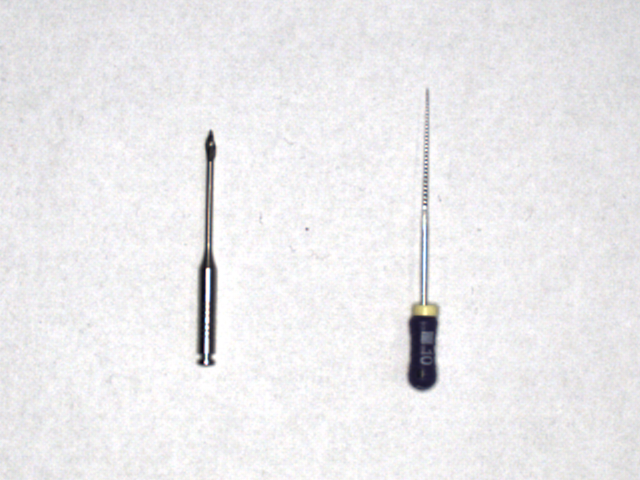
\includegraphics[width=0.7\linewidth]{addOns/input_1.png}}\\
  \captionof{figure}{Mèches à détecter}
  \label{fig.Input1}
\end{minipage}\\
\vspace{0.2cm}

Le problème vient du fait qu'il peut y avoir plusieurs objets à l'écran dont la position et l'alignement est aléatoire. On se restreindra à une détection de 5 objets au maximum, mais le programme doit être facilement modulable pour changer cette valeur maximum en ne changeant qu'une seule variable.

\vspace{0.2cm}
\noindent
\begin{minipage}[c]{\textwidth}
  \centering
  \makebox[\textwidth]{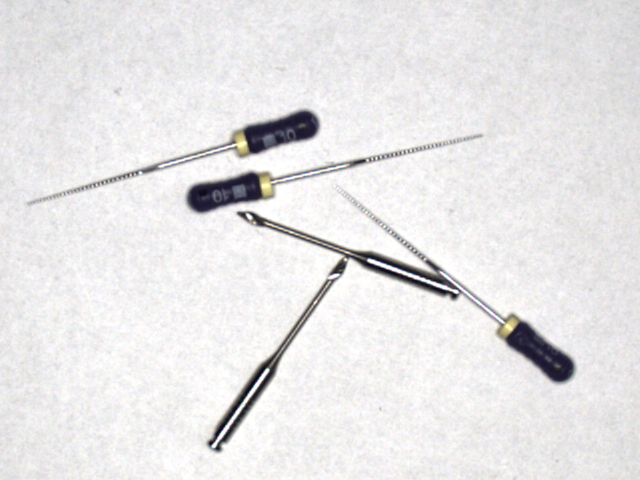
\includegraphics[width=0.7\linewidth]{addOns/input_2.png}}\\
  \captionof{figure}{Mèches à détecter dans un arrangement aléatoire}
  \label{fig.Input2}
\end{minipage}\\
\vspace{0.2cm}


\newpage
\subsection{Résultats attendus}
\noindent Il faut que le programme :
\begin{itemize}
  \item affiche en haut à gauche les types des objets détectés,
  \item affiche à la position de l'objet le numéro de l'objet,
  \item affiche une flèche sur chaque objet orientée dans la direction détectée, de longueur adaptée au type d'objet et de couleur spécifique à l'objet.
\end{itemize}

\vspace{0.2cm}
\noindent
\begin{minipage}[c]{\textwidth}
  \centering
  \makebox[\textwidth]{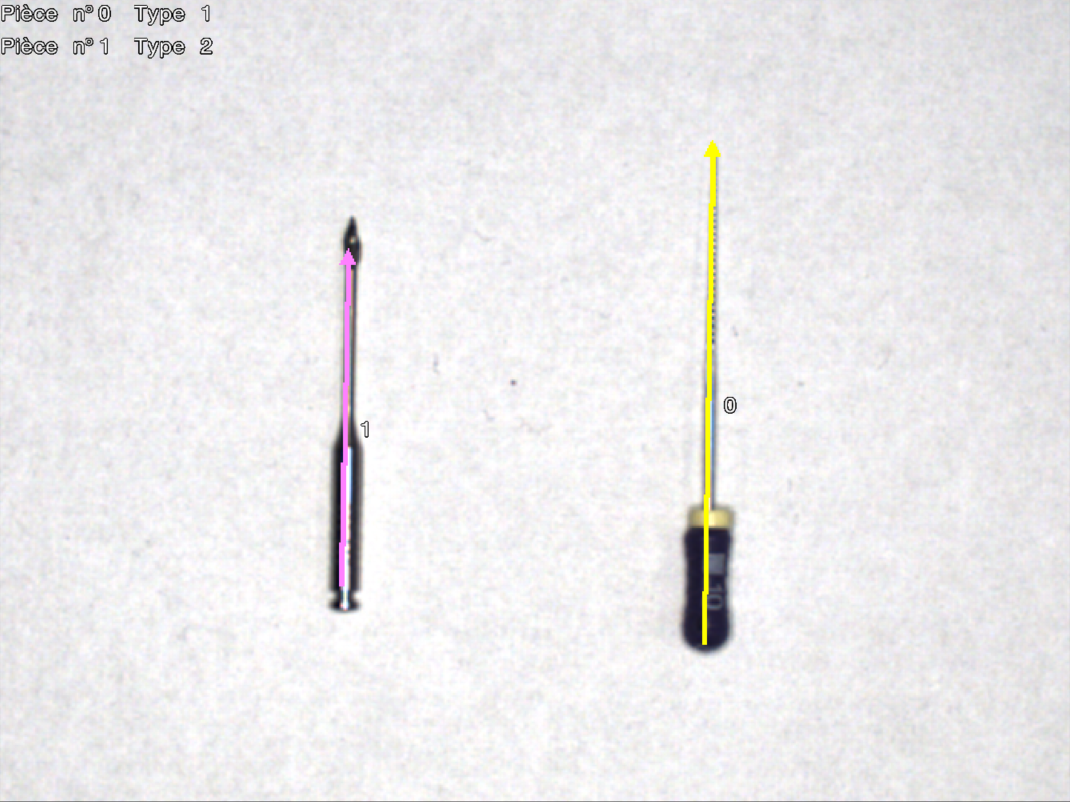
\includegraphics[width=0.7\linewidth]{addOns/output_1.png}}\\
  \captionof{figure}{Résultats attendus}
  \label{fig.Resultats}
\end{minipage}\\

\vspace{0.2cm}
\noindent
\begin{minipage}[c]{\textwidth}
  \centering
  \makebox[\textwidth]{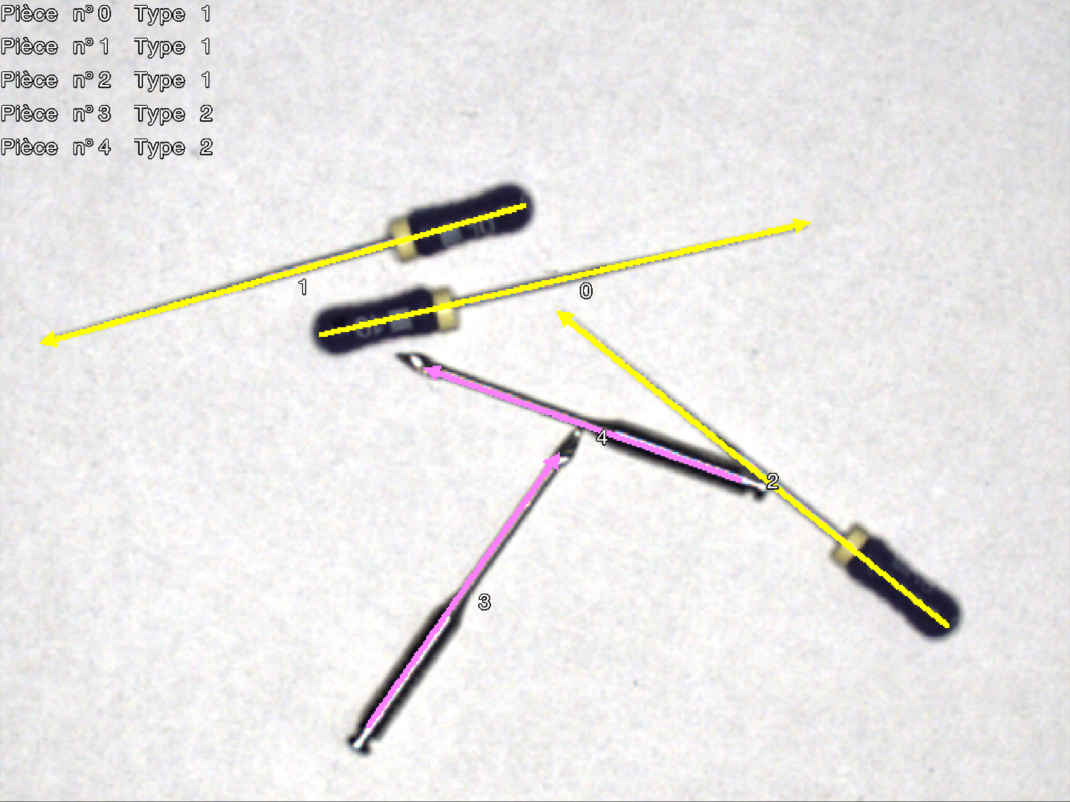
\includegraphics[width=0.7\linewidth]{addOns/output_2.png}}\\
  \captionof{figure}{Résultats attendus}
  \label{fig.Resultats}
\end{minipage}\\
